\documentclass[12pt,twoside]{report}

% some definitions for the title page
\newcommand{\reporttitle}{A Virtual Volumetric Screen}
\newcommand{\reportauthor}{Mr Robert Searby Buxton}
\newcommand{\supervisor}{Dr Nicole Salomons}
\newcommand{\reporttype}{MEng Individual Project}
\newcommand{\degreetype}{Computing MEng}  

% load some definitions and default packages
%%%%%%%%%%%%%%%%%%%%%%%%%%%%%%%%%%%%%%%%%
% University Assignment Title Page 
% LaTeX Template
% Version 1.0 (27/12/12)
%
% This template has been downloaded from:
% http://www.LaTeXTemplates.com
%
% Original author:
% WikiBooks (http://en.wikibooks.org/wiki/LaTeX/Title_Creation)
%
% License:
% CC BY-NC-SA 3.0 (http://creativecommons.org/licenses/by-nc-sa/3.0/)
% 
%
%%%%%%%%%%%%%%%%%%%%%%%%%%%%%%%%%%%%%%%%%
%----------------------------------------------------------------------------------------
%	PACKAGES AND OTHER DOCUMENT CONFIGURATIONS
%----------------------------------------------------------------------------------------
\usepackage[usenames,dvipsnames]{xcolor}
\usepackage[a4paper,hmargin=2.0cm,vmargin=2.0cm,includeheadfoot]{geometry}
\usepackage{textpos}
\usepackage[style=numeric, backend=biber]{biblatex} % for bibliography
\usepackage{csquotes}
\usepackage{tabularx,longtable,multirow,subfigure,caption}%hangcaption
\usepackage{fancyhdr} % page layout
\usepackage{url} % URLs
\usepackage[english]{babel}
\usepackage{amsmath}
\usepackage{graphicx}
\usepackage{svg}
\usepackage[many,minted]{tcolorbox}
\usepackage{epstopdf} % automatically replace .eps with .pdf in graphics
\usepackage{array}
\usepackage{latexsym}
\usepackage[pdftex,hypertexnames=false,colorlinks]{hyperref} % provide links in pdf
\usepackage{opensans}
\usepackage{float}
\usepackage{adjustbox}
\usepackage{listings}
\usepackage{fontspec}
\usepackage[all]{hypcap}
\usepackage{enumitem}

\addbibresource{references.bib}

\hypersetup{pdftitle={},
  pdfsubject={},
  pdfauthor={},
  pdfkeywords={},
  pdfstartview=FitH,
  pdfpagemode={UseOutlines},% None, FullScreen, UseOutlines
  bookmarksnumbered=true, bookmarksopen=true, colorlinks,
  citecolor=black,%
  filecolor=black,%
  linkcolor=black,%
  urlcolor=black}


% Removes annoying errors
\hbadness=99999 


\setmainfont{XCharter}
\setmonofont{CMU Typewriter Text}
%%% Default fonts
% \renewcommand*{\rmdefault}{bch}
% \renewcommand*{\ttdefault}{cmtt}

%%% Default settings (page layout)
\setlength{\parindent}{0em}  % indentation of paragraph

\setlength{\parindent}{0em}  % indentation of paragraph

\setlength{\headheight}{14.5pt}
\pagestyle{fancy}
\renewcommand{\chaptermark}[1]{\markboth{\chaptername\ \thechapter.\ #1}{}}
%\fancyhead[RO]{\sffamily \textbf{\thepage}} %Page no.in the right on even pages
%\fancyhead[LE]{\sffamily \textbf{\thepage}} %Page no. in the left on odd pages

\fancyfoot[ER,OL]{\thepage}%Page no. in the left on
%odd pages and on right on even pages
\fancyfoot[OC,EC]{\sffamily }
\renewcommand{\headrulewidth}{0.1pt}
\renewcommand{\footrulewidth}{0.1pt}
\captionsetup{margin=10pt,font=small,labelfont=bf}


%--- chapter heading

\def\@makechapterhead#1{%
  \vspace*{10\p@}%
  {\parindent \z@ \raggedright \sffamily
    \interlinepenalty\@M
    \Huge\bfseries \thechapter \space\space #1\par\nobreak
    \vskip 30\p@
  }}

%--- chapter heading

\def\@makechapterhead#1{%
  \vspace*{10\p@}%
  {\parindent \z@ \raggedright \sffamily
    %{\Large \MakeUppercase{\@chapapp} \space \thechapter}
    %\\
    %\hrulefill
    %\par\nobreak
    %\vskip 10\p@
    \interlinepenalty\@M
    \Huge\bfseries \thechapter \space\space #1\par\nobreak
    \vskip 30\p@
  }}

%---chapter heading for \chapter*  
\def\@makeschapterhead#1{%
  \vspace*{10\p@}%
  {\parindent \z@ \raggedright
    \sffamily
    \interlinepenalty\@M
    \Huge \bfseries  #1\par\nobreak
    \vskip 30\p@
  }}
\allowdisplaybreaks

% load some macros
% Here, you can define your own macros. Some examples are given below.

% \newcommand{\R}[0]{\mathds{R}} % real numbers
% \newcommand{\Z}[0]{\mathds{Z}} % integers
% \newcommand{\N}[0]{\mathds{N}} % natural numbers
% \newcommand{\C}[0]{\mathds{C}} % complex numbers
% \renewcommand{\vec}[1]{{\boldsymbol{{#1}}}} % vector
% \newcommand{\mat}[1]{{\boldsymbol{{#1}}}} % matrix

\newcommand{\tocite}{{\color{red} \small ToCite }} % placeholder for later citation
\newcommand{\todo}{{\color{red} \small TODO }} % placeholder for later citation

\lstdefinestyle{tree}{
literate=
  {├}{{\smash{\raisebox{-1ex}{\rule{1pt}{\baselineskip}}}\raisebox{0.5ex}{\rule{1ex}{1pt}}}}1
{─}{{\raisebox{0.5ex}{\rule{1.5ex}{1pt}}}}1
{└}{{\smash{\raisebox{0.5ex}{\rule{1pt}{\dimexpr\baselineskip-1.5ex}}}\raisebox{0.5ex}{\rule{1ex}{1pt}}}}1
}

\newcommand{\nixstore}[2][1]{\textcolor{Purple}{\texttt{/nix/store/}}\textcolor{RoyalBlue}{\texttt{#1}-}\textcolor{Orange}{\texttt{#2}}}

\newcommand{\mynewminted}[3]{%
  \newminted[#1]{#2}{#3}%
  \tcbset{myminted/#1/.style={minted language=#2,minted options={#3}}}}


%Programming Languages
\mynewminted{nix}{nix}{
  breaklines,
  linenos,
  autogobble,
  numbersep=2mm,
  fontsize=\footnotesize,
  frame=none}

\mynewminted{cpp}{cpp}{
  breaklines,
  linenos,
  autogobble,
  numbersep=2mm,
  fontsize=\footnotesize,
  frame=none}

\mynewminted{shell}{shell}{
  breaklines,
  autogobble,
  fontsize=\footnotesize,
  frame=none}


\newtcbinputlisting[auto counter,number within=section,list inside=mypyg]{\codeBoxFile}[4][]{%
  center,
  listing engine=minted,
  listing only,
  title={{\color{Black} \textbf{Listing \thetcbcounter:}} {\small #4}},
  % list entry={\protect\numberline{\thetcbcounter}#3},
  listing file={#3},
  enhanced jigsaw,
  breakable,
  colframe = Apricot!25,
  colback  = Apricot!10,
  coltitle = Apricot!20!black,
  drop fuzzy shadow,
  before skip = 20pt,
  after skip = 20pt,
  myminted/#2,
  #1}

%Boxes
\newtcolorbox[auto counter,number within=section]{figureBox}[2][]
{
  center,
  enhanced jigsaw,
  breakable,
  colframe = Apricot!25,
  colback  = Apricot!10,
  coltitle = Apricot!20!black,
  drop fuzzy shadow,
  title    = {{\color{Black} \textbf{Figure \thetcbcounter:}} {\small #2}},
  before skip = 20pt,
  after skip = 20pt,
  before upper={\centering \color{Gray!20!black}},
  #1,
}

\newtcbox[auto counter,number within=section]{\pictureBox}[2][]
{
  enhanced jigsaw,
  nobeforeafter,
  colframe = Apricot!25,
  colback= Apricot!25,
  coltitle = Apricot!20!black,
  drop fuzzy shadow,
  boxsep=3pt,
  left=0pt,
  right=0pt,
  top=0pt,
  bottom=0pt,
  title    = {{\color{Black} \textbf{Figure \thetcbcounter:}} {\small #2}},
  #1,
}

%Invisible box

\newtcolorbox{invisBox}{
  center,
  enhanced jigsaw,
  breakable,
  before skip=20pt,
  after skip=20pt,
  left=0pt,
  right=0pt,
  top=0pt,
  bottom=0pt,
  colframe=white, % Frame color
  colback=white,  % Background color
  opacityframe=0, % Frame opacity
  opacityback=0   % Background opacity
}

% load title page
\begin{document}
% !TEX root = ./main.tex

% Last modification: 2015-08-17 (Marc Deisenroth)
\begin{titlepage}

\newcommand{\HRule}{\rule{\linewidth}{0.5mm}} % Defines a new command for the horizontal lines, change thickness here

%----------------------------------------------------------------------------------------
%	LOGO SECTION
%----------------------------------------------------------------------------------------


\includegraphics[width = 4cm]{./figures/imperial}\\[0.5cm] 

\center % Center everything on the page
 
%----------------------------------------------------------------------------------------
%	HEADING SECTIONS
%----------------------------------------------------------------------------------------

\textsc{\LARGE \reporttype}\\[1.5cm] 
\textsc{\Large Department of Computing}\\[0.5cm] 
\textsc{\large Imperial College of Science, Technology and Medicine}\\[0.5cm] 

%----------------------------------------------------------------------------------------
%	TITLE SECTION
%----------------------------------------------------------------------------------------

\HRule \\[0.4cm]
{ \huge \bfseries \reporttitle}\\ % Title of your document
\HRule \\[1.5cm]
 
%----------------------------------------------------------------------------------------
%	AUTHOR SECTION
%----------------------------------------------------------------------------------------

\begin{minipage}{0.4\textwidth}
\begin{flushleft} \large
\emph{Author:}\\
\reportauthor % Your name
\end{flushleft}
\end{minipage}
~
\begin{minipage}{0.4\textwidth}
\begin{flushright} \large
\emph{Supervisor:} \\
\supervisor % Supervisor's Name
\end{flushright}
\end{minipage}\\[4cm]




%----------------------------------------------------------------------------------------


%----------------------------------------------------------------------------------------
%	DATE SECTION
%----------------------------------------------------------------------------------------

{\large \today} % Date, change the \today to a set date if you want to be precise


\vfill % Fill the rest of the page with whitespace
Submitted in partial fulfillment of the requirements for the \degreetype~of Imperial College London

\end{titlepage}



% page numbering etc.
\pagenumbering{roman}
\clearpage{\pagestyle{empty}\cleardoublepage}
\setcounter{page}{1}
\pagestyle{fancy}

%%%%%%%%%%%%%%%%%%%%%%%%%%%%%%%%%%%%
\begin{abstract}
Your abstract.
\end{abstract}

\cleardoublepage
%%%%%%%%%%%%%%%%%%%%%%%%%%%%%%%%%%%%
\section*{Acknowledgments}
Comment this out if not needed.

\clearpage{\pagestyle{empty}\cleardoublepage}

%%%%%%%%%%%%%%%%%%%%%%%%%%%%%%%%%%%%
%--- table of contents
\fancyhead[RE,LO]{\sffamily {Table of Contents}}
\tableofcontents 


\clearpage{\pagestyle{empty}\cleardoublepage}
\pagenumbering{arabic}
\setcounter{page}{1}
\fancyhead[LE,RO]{\slshape \rightmark}
\fancyhead[LO,RE]{\slshape \leftmark}

%%%%%%%%%%%%%%%%%%%%%%%%%%%%%%%%%%%%
\chapter{Introduction}

\begin{figure}[tb]
\centering

\includegraphics[width = 0.4\hsize]{./figures/imperial}
\caption{Imperial College Logo. It's nice blue, and the font is quite stylish. But you can choose a different one if you don't like it.}
\label{fig:logo}
\end{figure}

Figure~\ref{fig:logo} is an example of a figure. 

%%%%%%%%%%%%%%%%%%%%%%%%%%%%%%%%%%%%
\chapter{Background}
\newpage

\section{Nix/NixOS}
\subsection{Introduction to Nix}

\textbf{Nix} \cite{dolstra2004nix} is an open-source, "purely functional package manager” used in Unix-like operating systems to provide a functional and reproducible approach to package management. Started in 2003 as a research project Nix \cite{dolstra2006purely} is widely used in both industry \cite{NixCommunityNixOSWiki} and academia \cite{10.1145/3152493.3152556} \cite{https://doi.org/10.1002/qua.26872} \cite{LHCbNix}, and its associated public package repository \texttt{nixpkgs} \cite{NixPkgs} as of Jan 2024 has over 80,000 unique packages making it the largest up-to-date package repository in the world  \cite{Marakasov_2024}. Out of Nix has also grown \textbf{NixOS} \cite{10.1145/1411204.1411255} a Linux distribution that is conceived and defined as a deterministic and reproducible entity that is declared functionally and is built using the \textbf{Nix} package manager. \\

Nix packages are defined in the \textbf{Nix Language} a lazy functional programming language where packages are treated like purely functional values that are built by side effect-less functions and once produced are immutable. Packages are built with every dependency down to the \texttt{ELF} interpreter and \texttt{libc} (C standard library) defined in nix. All packages are installed in the store directory, typically \texttt{/nix/store/} by their unique hash and package name as can be seen in Fig~\ref{fig:nix-store-path} as opposed to the traditional Unix Filesystem Hierarchy Standard (FHS).

%% Nix Store Path
\begin{figureBox}[label={fig:nix-store-path}, width=0.8\linewidth]{Nix Store Path}
  \begin{tabbing}
    \={\color{Purple}\texttt{/nix/store/}}\={\color{RoyalBlue}\texttt{sbldylj3clbkc0aqvjjzfa6slp4zdvlj}}-\={\color{Orange}\texttt{hello-2.12.1}} \\
    \>\small{Prefix} \>\small {Hash part} \>\small {Package name}
  \end{tabbing}
\end{figureBox}

Package source files, like tarballs and patches, are also downloaded and stored with their hash in the store directory where packages can find them when building. Changing a package's dependencies results in a different hash and therefore location in the store directory which means you can have multiple versions or variants of the same package installed simultaneously without issue. This design also avoids "DLL hell" by making it impossible to accidentally point at the wrong version of a package. Another important result is that upgrading or uninstalling a package cannot ever break other applications. \\

Nix builds packages in a sandbox to ensure they are built exactly the same way on every machine by restricting access to nonreproducible files, OS features (like time and date), and the network \cite{nixcon-sandboxs}. A package can and should be pinned to a specific NixOS release (regardless of whether you are using NixOS or just the package manager). This means that once a package is configured to build correctly it will continue to work the same way in the future, regardless of when and where it is used and it will never not be able to be built. \\

These features are extremely useful for scientific work, CERN uses Nix to package the LHCb Experiment because it allows the software "to be stable for long periods (longer than even long-term support operating systems)" and it means that as Nix is reproducible; all the experiments are completely reproducible as all bugs that existed in the original experiment stay and ensure the accuracy of the results \cite{LHCbNix}. \\

To create a package Nix evaluates a \textbf{derivation} which is a specification/recipe that defines how a package should be built. It includes all the necessary information and instructions for building a package from its source code, such as the source location, build dependencies, build commands, and post-installation steps. By default, Nix uses binary caching to build packages faster, the default cache is \texttt{cache.nixos.org} is open to everyone and is constantly being populated by CI systems. You can also specify custom caches. The basic iterative process for building Nix packages can be seen in Fig~\ref{fig:nix-derivation-loop}.

\begin{figureBox}[label = {fig:nix-derivation-loop}, width=0.8\linewidth]{Nix Build Loop}
  { \footnotesize
  \begin{enumerate}
    \item A hash is computed for the package derivation and, using that hash, a Nix store path is generated, e.g \nixstore[sbldylj3clbkc0aqvjjzfa6slp4zdvlj]{hello-2.12.1}.
    \item  Using the store path, Nix checks if the derivation has already been built. First, checking the configured Nix store e.g {\color{Purple}\texttt{/nix/store/}} to see if the path e.g {\color{RoyalBlue}\texttt{sbldylj3clbkc0aqvjjzfa6slp4zdvlj}}-{\color{Orange}\texttt{hello-2.12.1}} already exists. If it does, it uses that, if it does not it continues to the next step.
    \item Next it checks if the store path exists in a configured binary cache, this is by default \texttt{cache.nixos.org}. If it does it downloads it from the cache and uses that. If it does not it continues to the next step.
    \item Nix will build the derivation from scratch, recursively following all of the steps in this list, using already-realized packages whenever possible and building only what is necessary. Once the derivation is built, it is added to the Nix store.
  \end{enumerate}
  }
\end{figureBox}

\subsection{Example of a Nix package}

To give an example of what a Nix package might look like. We have created a flake (one method of defining a package) in Listing~\ref{list:nix-flake} that builds a version of the classic example package "hello". 

\codeBoxFile[label = {list:nix-flake}]{nix}{./background/code/hello.nix}{flake.nix}

To dive deeper into what each line does we have given a breakdown below for the \texttt{flake.nix} \\
{ \small
\begin{itemize}
  \item \textbf{Line 2:} We have specified that we want to build our flake with the stable \textbf{nix channel} \texttt{nixos-23.11}, the most recent channel at the time of writing. This "channel" is just a release branch on the \texttt{nixpkgs} GitHub repository. Channels do receive conservative updates such as bug fixes and security patches but no major updates after the initial release. The first time we build the hello package from our \texttt{flake.nix} a \texttt{flake.lock} is automatically generated that pins us to a specific revision of \texttt{nixos-23.11}. Our built inputs will not change until we relock our flake to either a different revision of \texttt{nixos-23.11} or a new channel entirely. 

  \item \textbf{Line 5:} Here we define \texttt{outputs} as a function that accepts, \texttt{self} (the flake) and \texttt{nixpkgs} (the set of packages we just pinned to on line 2). Nix will resolve all inputs, and then call the \texttt{output} function.
  
  \item \textbf{Line 6:} Here we specify that we are defining the default package for users on \texttt{x86\_64-linux}. If we tried to build this package on a different CPU architecture like for example ARM (\texttt{aarch64-linux}) the flake would refuse to build as the package has not been defined for ARM yet. If we desired we could fix this by adding a \texttt{defaultPackage.aarch64-linux} definition.

  \item \textbf{Line 7-9:} Here we are just defining a shorthand way to refer to x86 Linux packages. This syntax is similar if not identical to Haskell.

  \item \textbf{Line 10:} Here we begin the definition of the derivation which is the instruction set Nix uses to build the package.
  
  \item \textbf{Line 14:} We specify here that we need \texttt{gcc} in our sandbox to build our package. \texttt{gcc} here is shorthand for \texttt{gcc12} but we could specify any c compiler with any version of that compiler we liked. If you desired you could compile different parts of your package with different versions of GCC.

  \item \textbf{Line 15:} Here we are slightly abusing the configure phase to generate a hello.c file. You would usually download a source to build from with a command like \texttt{fetchurl} while providing a hash. Each phase is essentially run as a bash script. Everything inside \texttt{mkDerivation} is happening inside a sandbox that will be discarded once the package is built (technically after we garbage collect). 
  
  \item \textbf{Line 16:} Here we actually build our package
  
  \item \textbf{Line 17:} In this line we copy the executable we have generated which is currently in the sandbox into the actual package we are producing which will be in the store directory \texttt{/nix/store}. 
\end{itemize}
}
Below we have given some examples of how to run and investigate our hello package in Listing~\ref{list:nix-terminal}.

\codeBoxFile[label = {list:nix-terminal},  width=0.75\linewidth]{shell}{./background/code/hello-nix.sh}{Terminal}

In Fig~\ref{fig:dependency-graph} we can see the package dependency graph of our \texttt{hello} package. We are only dependent on 4 packages \texttt{libunistring}, \texttt{libidn2}, \texttt{xgcc}, \texttt{glibc} all of which Nix have installed and configured separately the rest of the non-nix system (assuming we are not on NixOS). 

\begin{figureBox}[label = {fig:dependency-graph}, width=0.75\linewidth]{Dependency graph}
  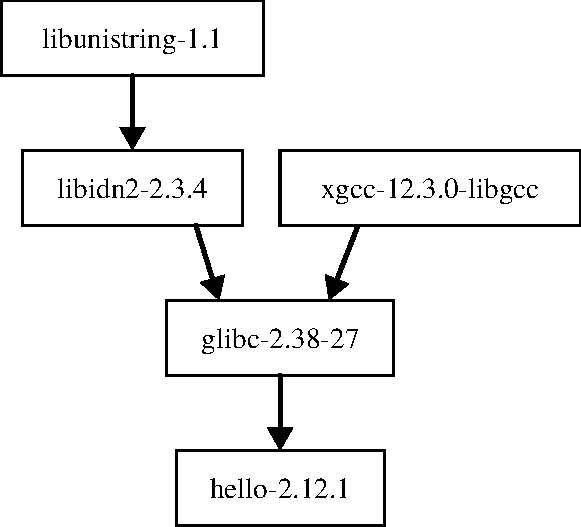
\includegraphics[width=0.7\linewidth]{./background/figures/nix/hello-pkg.pdf}
\end{figureBox}

\section{Perspective Projection}

\begin{figureBox}[label={fig:ortho-vs-persp}, width=0.8\linewidth]{Orthographic and perspective projections}
    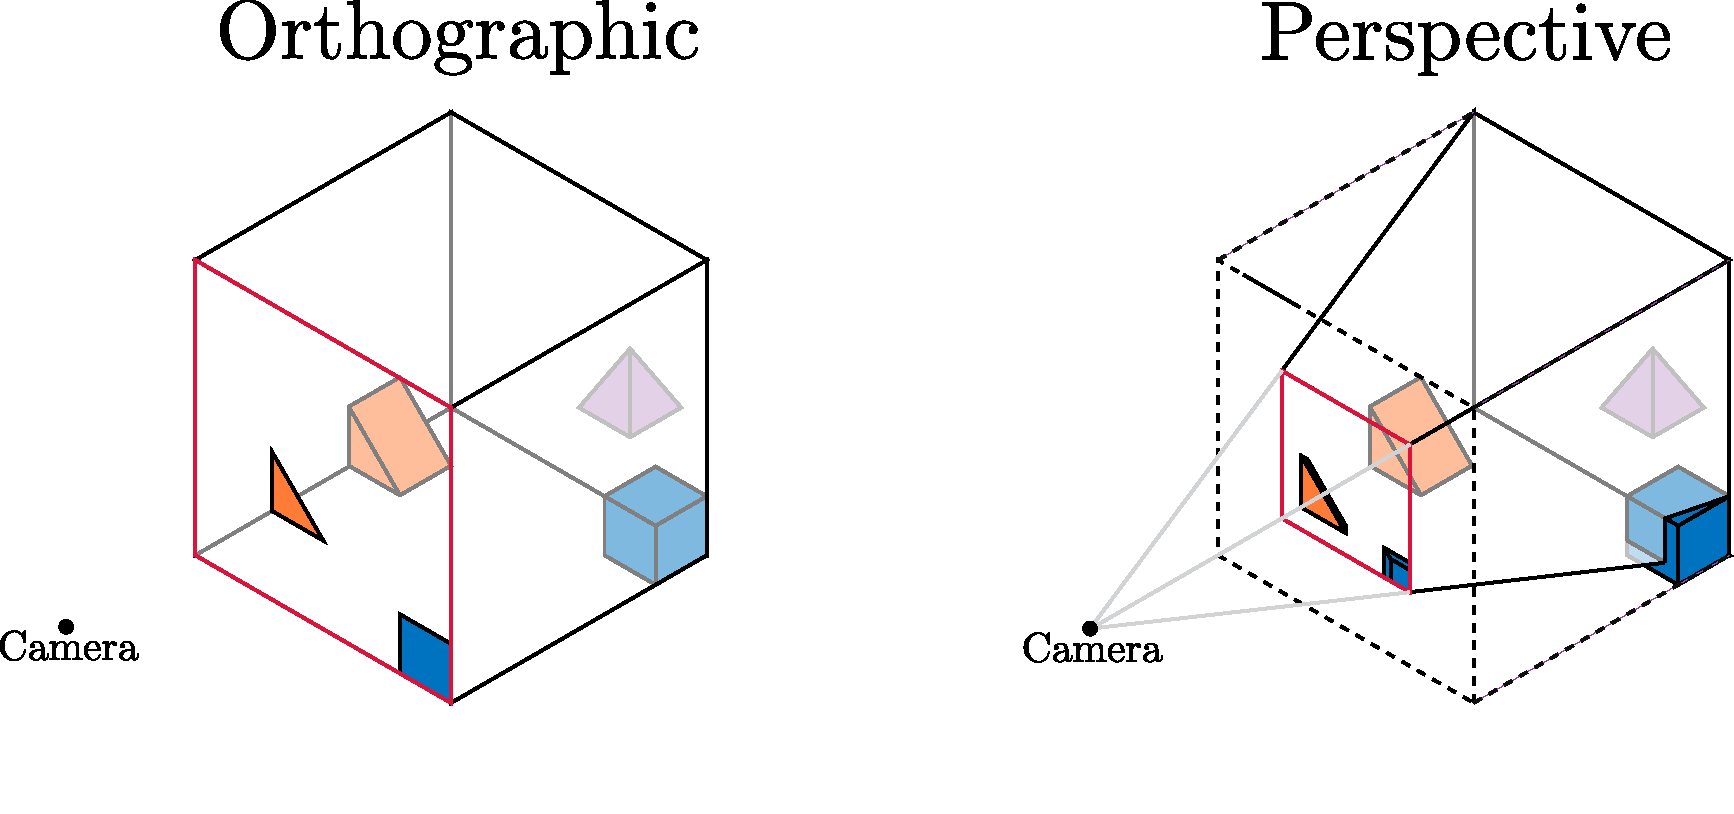
\includegraphics[width = 0.8\linewidth]{./background/figures/projection/ortho-vs-persp.pdf}
\end{figureBox}

To represent 3D objects on a 2D surface (our screen) OpenGL supports two types of projections: perspective and orthographic as seen in Fig~\ref{fig:ortho-vs-persp}. Orthographic features parallel projection lines (orthogonal to the projection plane), which means that it does not depict the effect of perspective. Distances are preserved, making it useful for technical drawings where measurements need to be precise and not skewed by perspective (All diagrams in this report are from the orthographic perspective). Unlike orthographic projection, perspective projection simulates the way the human eye perceives the world, with objects appearing smaller as they are farther from the viewpoint as the projection lines converge at a vanishing point. To create the illusion of 3D in this project we must use a perspective projection.

\subsection{Generating the perspective projection}

\begin{figureBox}[label={fig:persp-projection}, width=0.8\linewidth]{Using frustum to generate a perspective projection}
    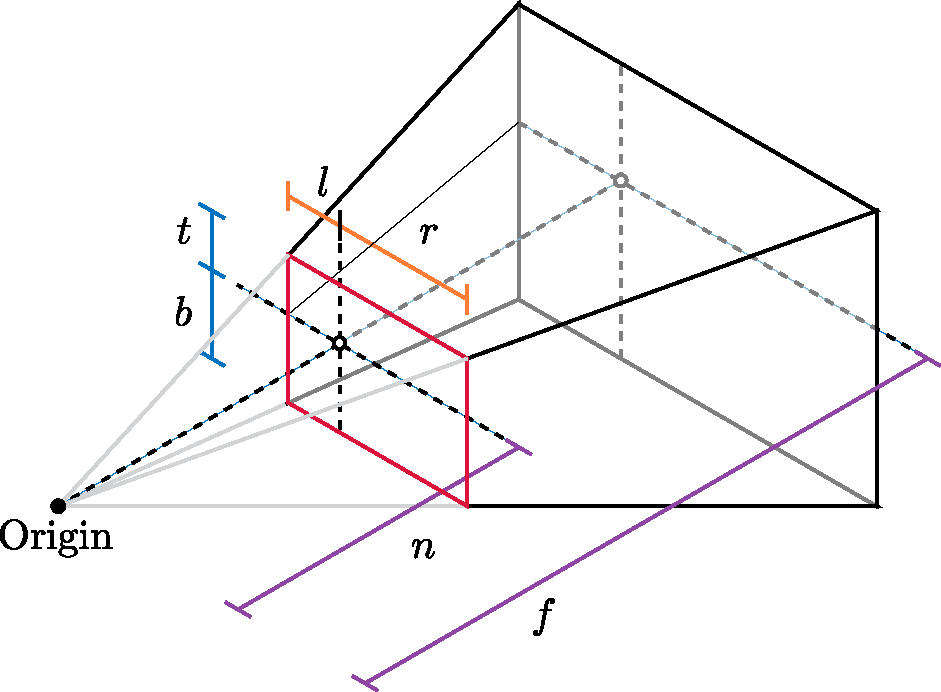
\includegraphics[width = 0.8\linewidth]{./background/figures/projection/persp-projection.pdf}
\end{figureBox}

OpenGL provides the \texttt{frustum} function as seen in Fig~\ref{fig:persp-projection} which can be used to construct a perspective matrix.     
\[
    \begin{bmatrix}
        \frac{2n}{r-l} & 0              & \frac{r+l}{r-l}  & 0                \\
        0              & \frac{2n}{t-b} & \frac{t+b}{t-b}  & 0                \\
        0              & 0              & -\frac{f+n}{f-n} & -\frac{2fn}{f-n} \\
        0              & 0              & -1               & 0                \\
    \end{bmatrix}
\] 
This maps a specified viewing frustum screen-space (with intermediate steps handled by OpenGL) \cite{hearn2004computer}. The viewing frustum is specified by six parameters: $f$, $l$, $r$, $b$, $t$, $n$ which represent left, right, bottom, top, near, and far. These parameters define the sides of the near-clipping plane, highlighted in red, relative to the origin of the coordinate system. These parameters do not represent distances or magnitudes in a traditional sense but rather define the vectors from the center of the near-clipping plane to its edges. \\


The $l$ and $r$ parameters specify the horizontal boundaries of the frustum on the near-clipping plane, with left typically being a negative value and right a positive value, defining the extent to which the frustum extends to the left and right of the origin. Similarly, the $b$ and $t$ parameters determine the vertical boundaries, with the bottom often negative and the top positive, expressing the extent of the frustum below and above the origin. \\

The $n$ and $f$ parameters are scalar values that specify the distances from the origin to the near and far clipping planes along the view direction. Altering the value of $n$ will change the angles of the lines (or vectors) that connect the corners of the near plane to the eye, effectively changing the "field of view". Changing the value $f$ affects the range of depth that is captured within the scene. \\

If we can track the position of a viewer's eye in real time then we can create the illusion of a 3D scene behind and in front of a display using \texttt{frustum}. This can be done fairly trivially following Robert Kooima's method he sets out in "Generalized Perspective Projection" to calculate $f$, $l$, $r$, $b$, $t$, $n$ as the viewer's eye moves \cite{kooima2009generalized}. \\

To encode the position and size of the screen we take 3 points, $p_a$, $p_b$ and $p_c$ which represent the lower-left, lower-right and upper-left points of the screen respectively when viewed from the front on. These points are in tracker space, the coordinate system of the device we use to track the eyes. This point can be used to generate an orthonormal basis of the screen of $s_r$, $s_u$ and $s_n$ which represents the directions up, right and normal to the screen respectively as seen in Fig~\ref{fig:perspective-screen}. We can compute these values from the screen corners as follows:
\[s_r = \frac{p_b-p_a}{||p_b-p_a||} \quad s_u = \frac{p_c-p_a}{||p_c-p_a||} \quad s_n = \frac{s_r\times s_u}{||s_r \times s_u||}\]

\begin{figureBox}[label={fig:perspective-screen}, width=0.8\linewidth]{Defining a screen in 3D space}
    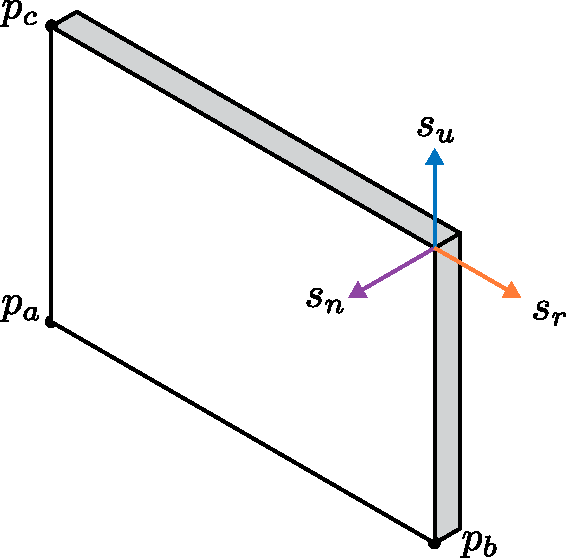
\includegraphics[width = 0.3\linewidth]{./background/figures/projection/screen.pdf}
\end{figureBox}

Introducing the viewer's eye which we will refer to as $p_e$. We can draw three vectors $v_a$, $v_b$, $v_c$ from the viewers eye $p_e$ to the corners of the screen $p_a$, $p_b$, $p_c$ as seen in Fig~\ref{fig:screen-extents}. In the diagram, we also have labeled the components of each of these vectors in the basis of the screen. We can compute these as follows:
\[ v_a = p_a - p_e \quad v_b = p_b - p_e \quad v_c = p_c - p_e\] 

To calculate the required values for \texttt{frustum} we must first find the point where a line drawn perpendicular to the plane of the screen that passes through $p_e$ strikes the plane of the screen. We refer to this point as the {\it screen-space-origin}, it is worth noting that this point can lie outside the screen (the rectangle bounded by $p_a$, $p_b$, $p_c$). We can find the distance of the {\it screen-space-origin} from the eye $p_e$ by taking its component of $v_a$, $v_b$, $v_c$ in the screen basis vector $s_n$, however, as $s_n$ is in the opposite direction we must invert it. Similarly, we can calculate $t$ by taking the component of $v_c$ in the basis vector $s_u$, $b$ by $v_b$ in $s_u$, $l$ by $v_c$ in $s_r$ and lastly $r$ by $v_b$ in $s_r$. We can compute these as follows:
\[ d= -(s_n \cdot v_a) \quad l = (v_c \cdot s_r) \quad r = (v_b \cdot s_r) \quad b = (v_c \cdot s_u) \quad t = (v_b \cdot s_u) \]

\begin{figureBox}[label={fig:screen-extents}, width=0.8\linewidth]{Screen Intersection with view}
    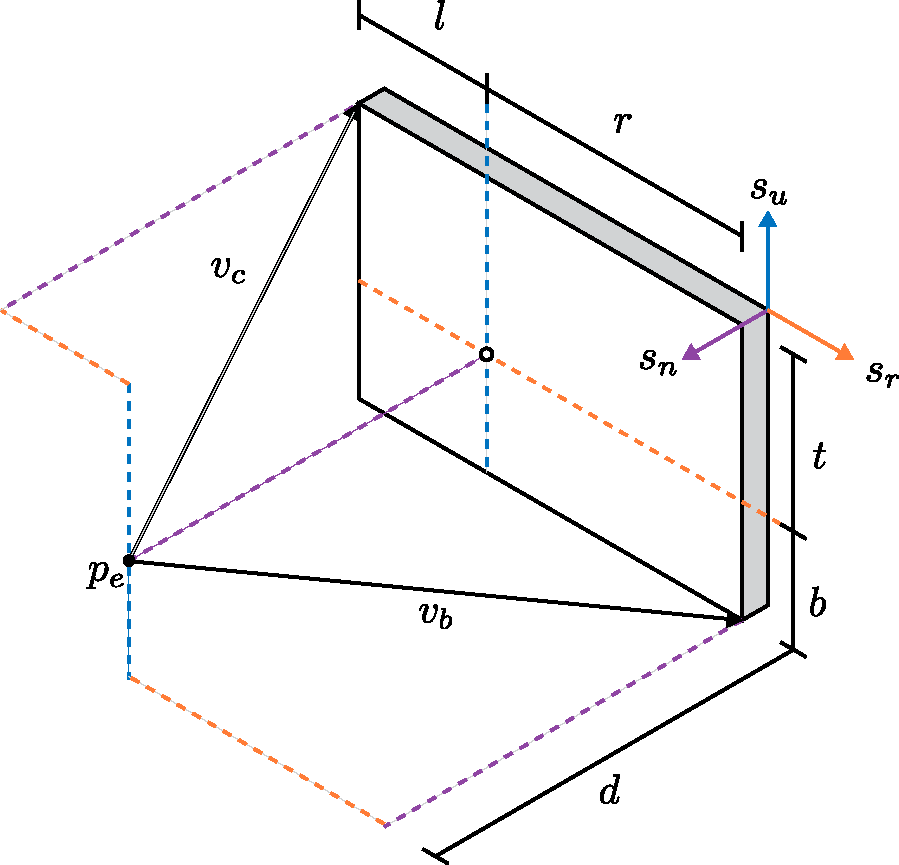
\includegraphics[width = 0.5\linewidth]{./background/figures/projection/eye-projection.pdf}
\end{figureBox}

We can now generate a projection matrix by calling \texttt{frustum} using $d$ as our near-clipping plane distance $n$ with an arbitrary value for the far-clipping plane $f$. Furthermore, we have now successfully generated our viewing frustum but we still have two problems. Firstly our frustum has been defined in tracker space so is pointed in the direction of our camera not the normal of our screen. We can remedy this problem by using a rotation matrix M to align our frustum with $s_n$, $s_u$ and $s_r$, the basis of our screen as seen in Fig~\ref{fig:basis-change}. M is defined as follows:
\[
    \begin{bmatrix}
        v_{rx} & v_{ry} & v_{rz} & 0 \\
        v_{ux} & v_{uy} & v_{uz} & 0 \\
        v_{nx} & v_{ny} & v_{nz} & 0 \\
        0      & 0      & 0      & 1 \\
    \end{bmatrix}
\]

\begin{figureBox}[label={fig:basis-change}, width=0.8\linewidth]{Moving the frustum from tracker space to screen space}
    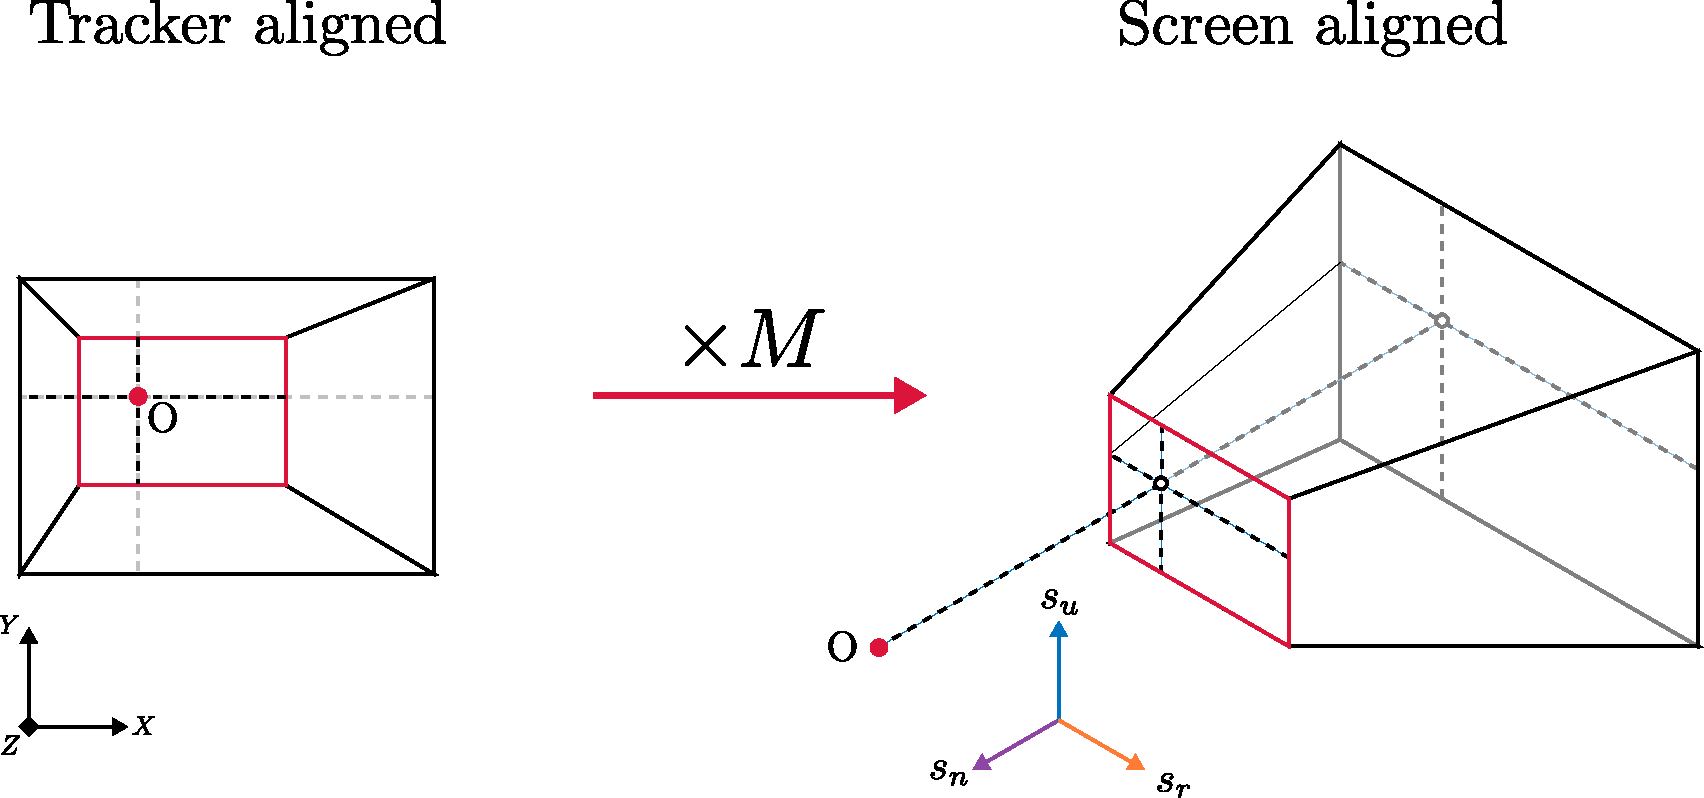
\includegraphics[width = 0.8\linewidth]{./background/figures/projection/realignment.pdf}
\end{figureBox}

The second problem we have is that we want our projection matrix to move around with the viewer's eye however the mathematics of perspective projection disallow this, with the camera forever trapped at the origin. To translate our viewing frustum to our eye position we must instead translate our eye position (and the whole world) to the apex/origin of our frustum. This can be done with a translation matrix $T$ as seen in Fig~\ref{fig:frust-translation}. $T$ can be generated with the OpenGL function \texttt{translate} where we want to offset it by the vector from our Origin to the viewers eye $p_e$. T is defined as follows:
\[
    \begin{bmatrix}
        1 & 0 & 0 & -p_{ex} \\
        0 & 1 & 0 & -p_{ey} \\
        0 & 0 & 1 & -p_{ez} \\
        0 & 0 & 0 & 1       \\
    \end{bmatrix}
\]

\begin{figureBox}[label={fig:frust-translation}, width=0.8\linewidth]{Translating the viewing frustum to sit inside the screen}
    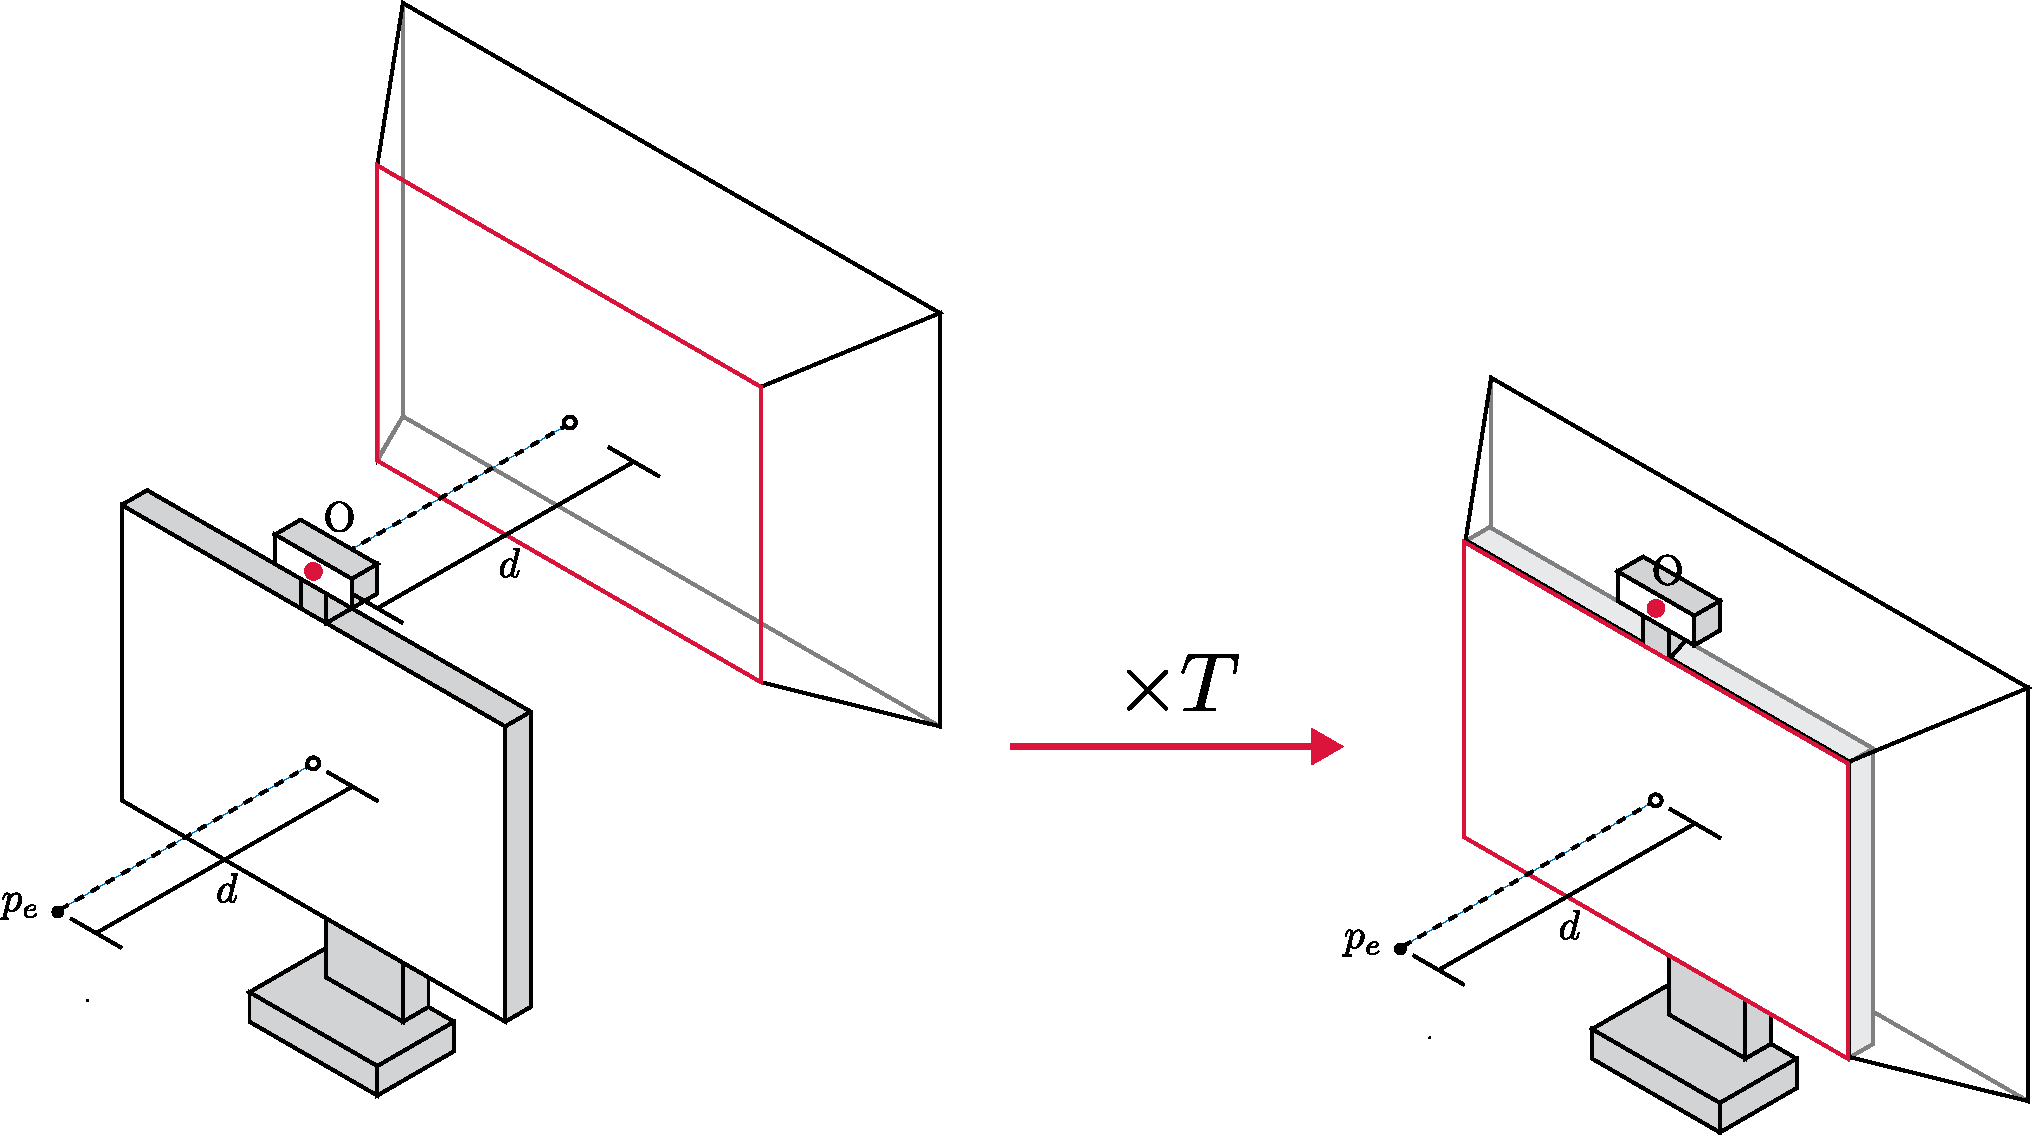
\includegraphics[width = 0.8\linewidth]{./background/figures/projection/frust-translation.pdf}
\end{figureBox}

We now have a working method for projecting virtual objects behind our screen onto our screen however it is also possible if we desire to project objects in front of the screen onto the screen as well as long as they lie within the pyramid formed between the edges of the screen and the viewer's eye. We can use similar triangles to scale the near-clipping plane from the plane of the screen to a small distance $n$ from our eye as seen in Fig~\ref{fig:extending-near}. Furthermore, we now have scaled-down values of $t$, $b$ $l$ and $r$ we can use for our new viewing frustum which we call $t_n$, $b_n$ $l_n$ and $r_n$. They are defined as follows:
\[
    l_n = (v_c \cdot s_r) \frac{n}{d} \quad r_n = (v_b \cdot s_r) \frac{n}{d} \quad b_n = (v_c \cdot s_u) \frac{n}{d} \quad t_n = (v_b \cdot s_u) \frac{n}{d}
\]

So our final viewing frustum takes in frustum extents $t_n$, $b_n$ $l_n$ and $r_n$ and $n$ and $f$ defining the distances to the near and far clipping plane.
\begin{figureBox}[label={fig:extending-near}, width=0.8\linewidth]{Extending the near plane to not clip out objects in front of the screen}
    \centering
    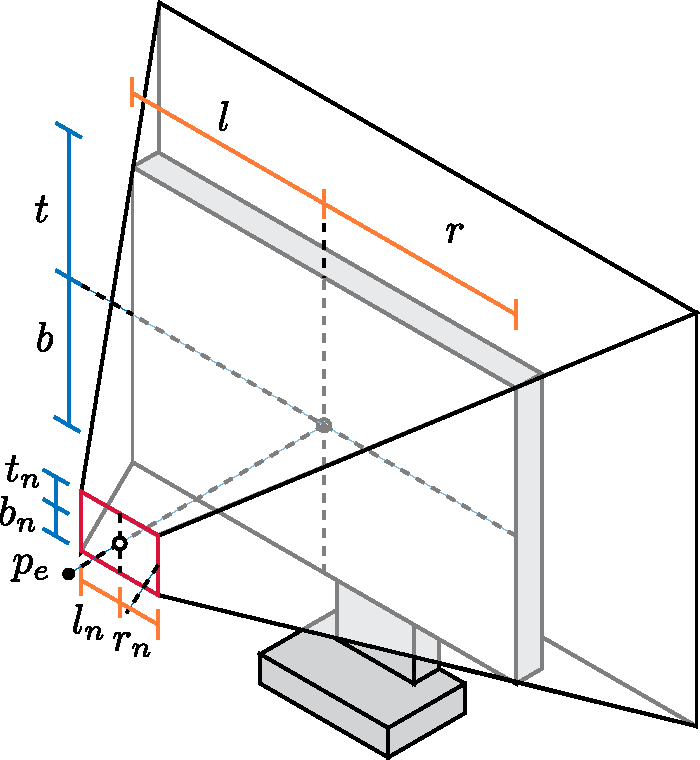
\includegraphics[width = 0.5\linewidth]{./background/figures/projection/extending-near.pdf}
\end{figureBox}

Following these steps, we can create an accurate projective providing the perspective we would expect to see if there was a scene in front and behind our screen. 

\subsection{Sample code}
Below we have attached some sample code of a function implementing the process we just described which is self-explanatory.

\codeBoxFile{cpp}{./background/code/projection.cpp}{projection.cpp, Sample code for creating the 3D illusion projection}

\section{Volumetric displays}

Volumetric displays \cite{1492264} provide a three-dimensional viewing experience by emitting light from each voxel, or volume element, in a 3D space. This approach enables the accurate representation of virtual 3D objects while providing accurate focal depth, motion parallax, and vergence. Vergence refers to the rotation of a viewer's eye to fixate on the same point they are focusing on. Moreover, volumetric displays allow multiple users to view the same display from different angles, providing unique perspectives of the same object simultaneously.

\subsection{Swept Volume Displays}
Swept volume displays are one prominent category of volumetric displays. They employ a moving 2D display to create a 3D image through the persistence of vision effects. This is achieved by moving the 2D display through a 3D space at high speeds while emitting light from the display where it reaches the position of each corresponding voxel. Common techniques for achieving this include using a rotating mirror \cite{10.1117/12.480930}, an emitting screen, typically an LED-based \cite{Gately:11}, or a transparent projector screen \cite{keane_volumetric_2016}. There currently exist commercial products that implement this technique as can be seen in Fig~\ref{fig:voxon} and Fig~\ref{fig:brightbox}.

\begin{invisBox}
  
  \pictureBox[label={fig:voxon}]{The VXR4612 3D Volumetric Display, a projector-based persistence of vision display produced by Voxon Photonics. \cite{voxon2}}{
    \adjustbox{height=4cm, keepaspectratio}{
      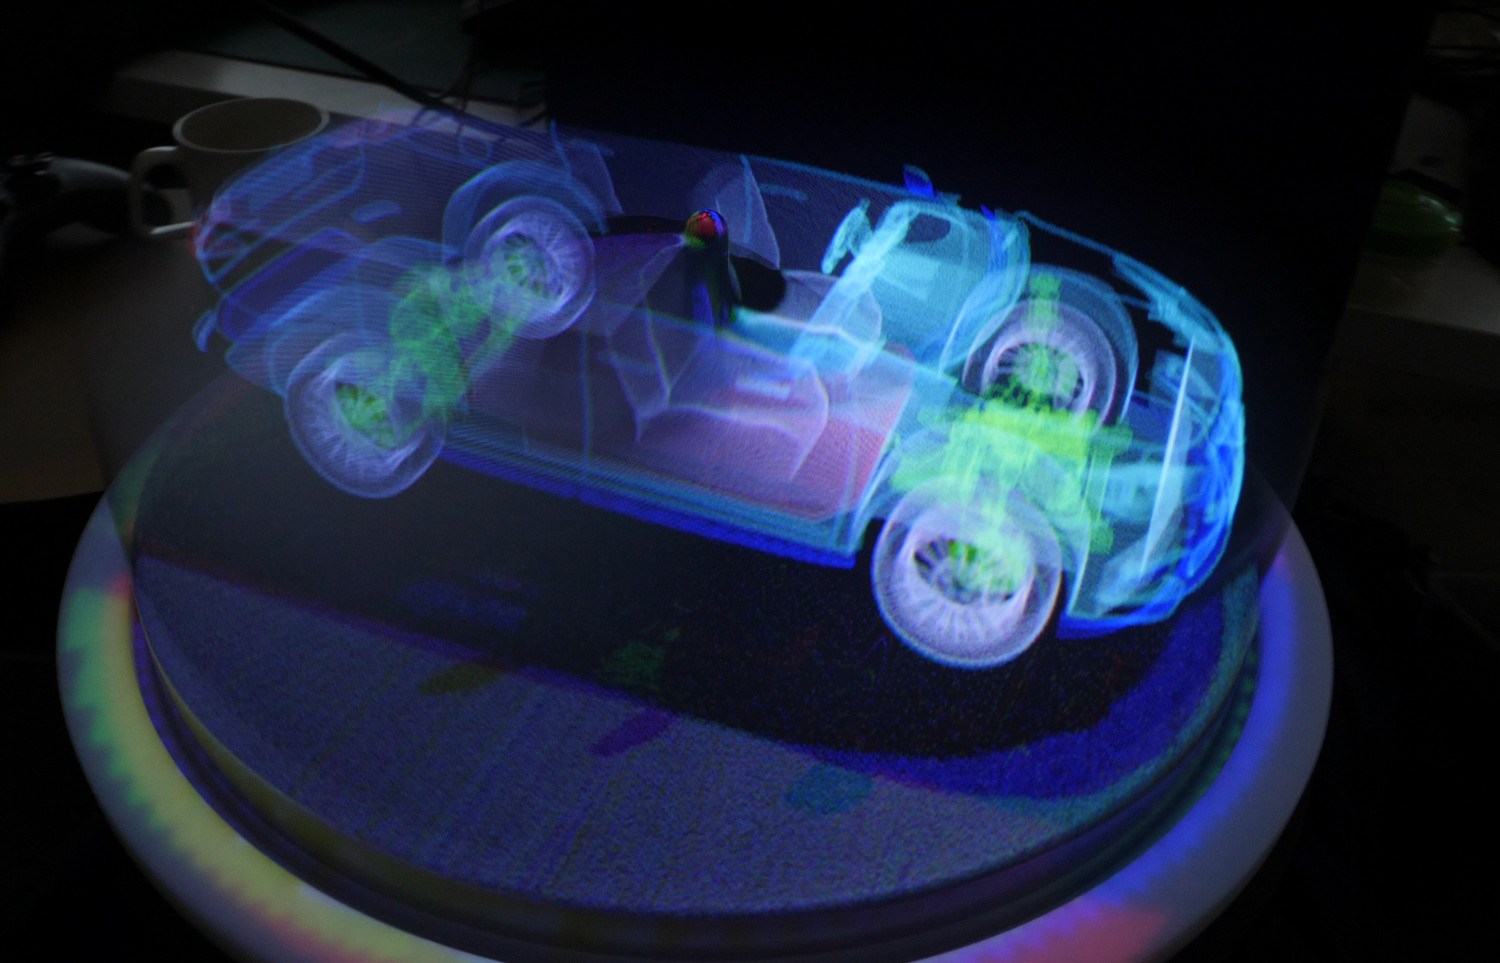
\includegraphics{./background/figures/3d/voxon.jpg}
    }
  }
  \hfill
  \pictureBox[label={fig:brightbox}]{A Volumetric Display / Holographic Signage, an LED-based persistence of vision display produced by Brightvox Inc. \cite{brightvox_2023}}{
  \adjustbox{height=4.5cm, keepaspectratio}{
    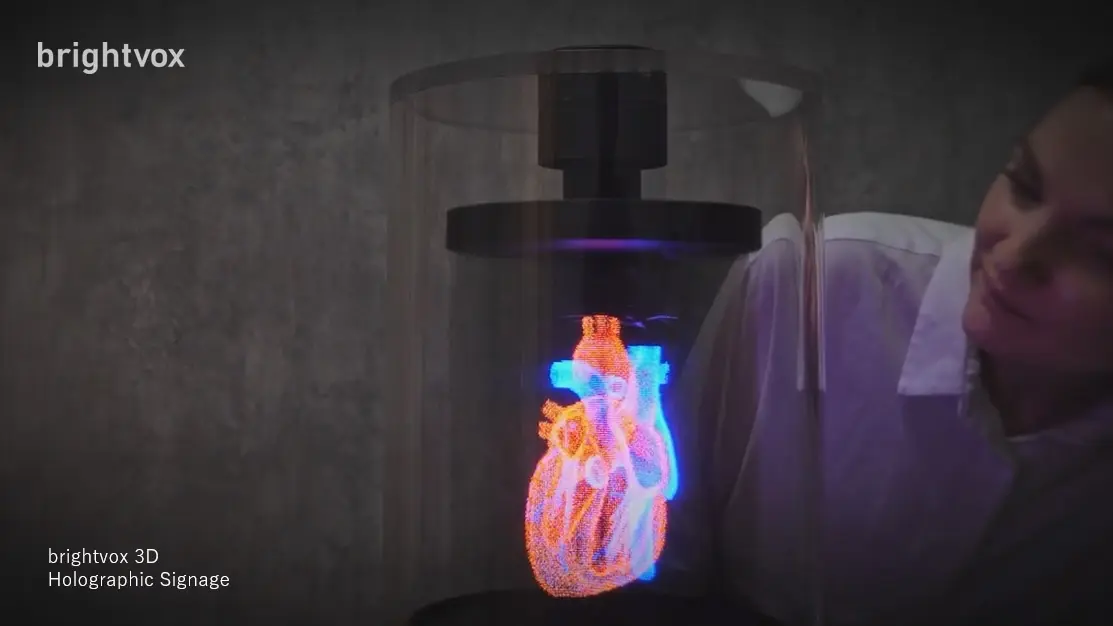
\includegraphics{./background/figures/3d/brightvox.png}
    }
  }
\end{invisBox}

\subsection{Static Volume Displays}
Static volume displays are another category. They employ a static transparent medium that when interacted with creates a 3D image. The result is that light is emitted from the display at each point in a 3D space. Techniques for achieving this range from using a 3D array of LEDs \cite{10.1145/2341931.2341937}, lasers and phosphorus gas \cite{https://doi.org/10.1002/anie.202003160}, or a transparent laser-induced damaged medium that can be projected into \cite{10.1145/1179849.1179982}. There has been research into photon-activated dye \cite{Patel2017} and even quantum dot-based displays \cite{Hirayama2015}. An example of one such display can be seen in Fig~\ref{fig:passive-optical}.

\subsection{Trapped Particle Displays}
Acoustic Trapping Displays displays are a relatively new category of volumetric displays. They employ a 3D array of particles that are suspended in air using acoustic levitation. \cite{10.1063/1.5113467} \cite{Hirayama2019} This is achieved by using an array of ultrasonic transducers to create a standing wave that can trap particles in the nodes of the wave. By moving the nodes of the wave through a 3D space and illuminating the particles with light, a 3D image can be created. This technique is still in its infancy and can struggle to provide a convincing persistence of vision effect. Another direction some researchers have taken is to use a photophoretic trap to trap particles in air \cite{Smalley2018}. The advantage of this sort of display is that space that is not being used to display an object is empty and can be passed through. This is in contrast to swept volume displays/most static volume displays where the space not being used to display an object is filled with the display's hardware. An example of one such display can be seen in Fig~\ref{fig:acoustic}.

\begin{invisBox}
	\pictureBox[label={fig:passive-optical}]{Columbia University's passive optical scattering volumetric display \cite{10.1145/1179849.1179982}}{
	  \adjustbox{height=5.25cm, keepaspectratio}{
		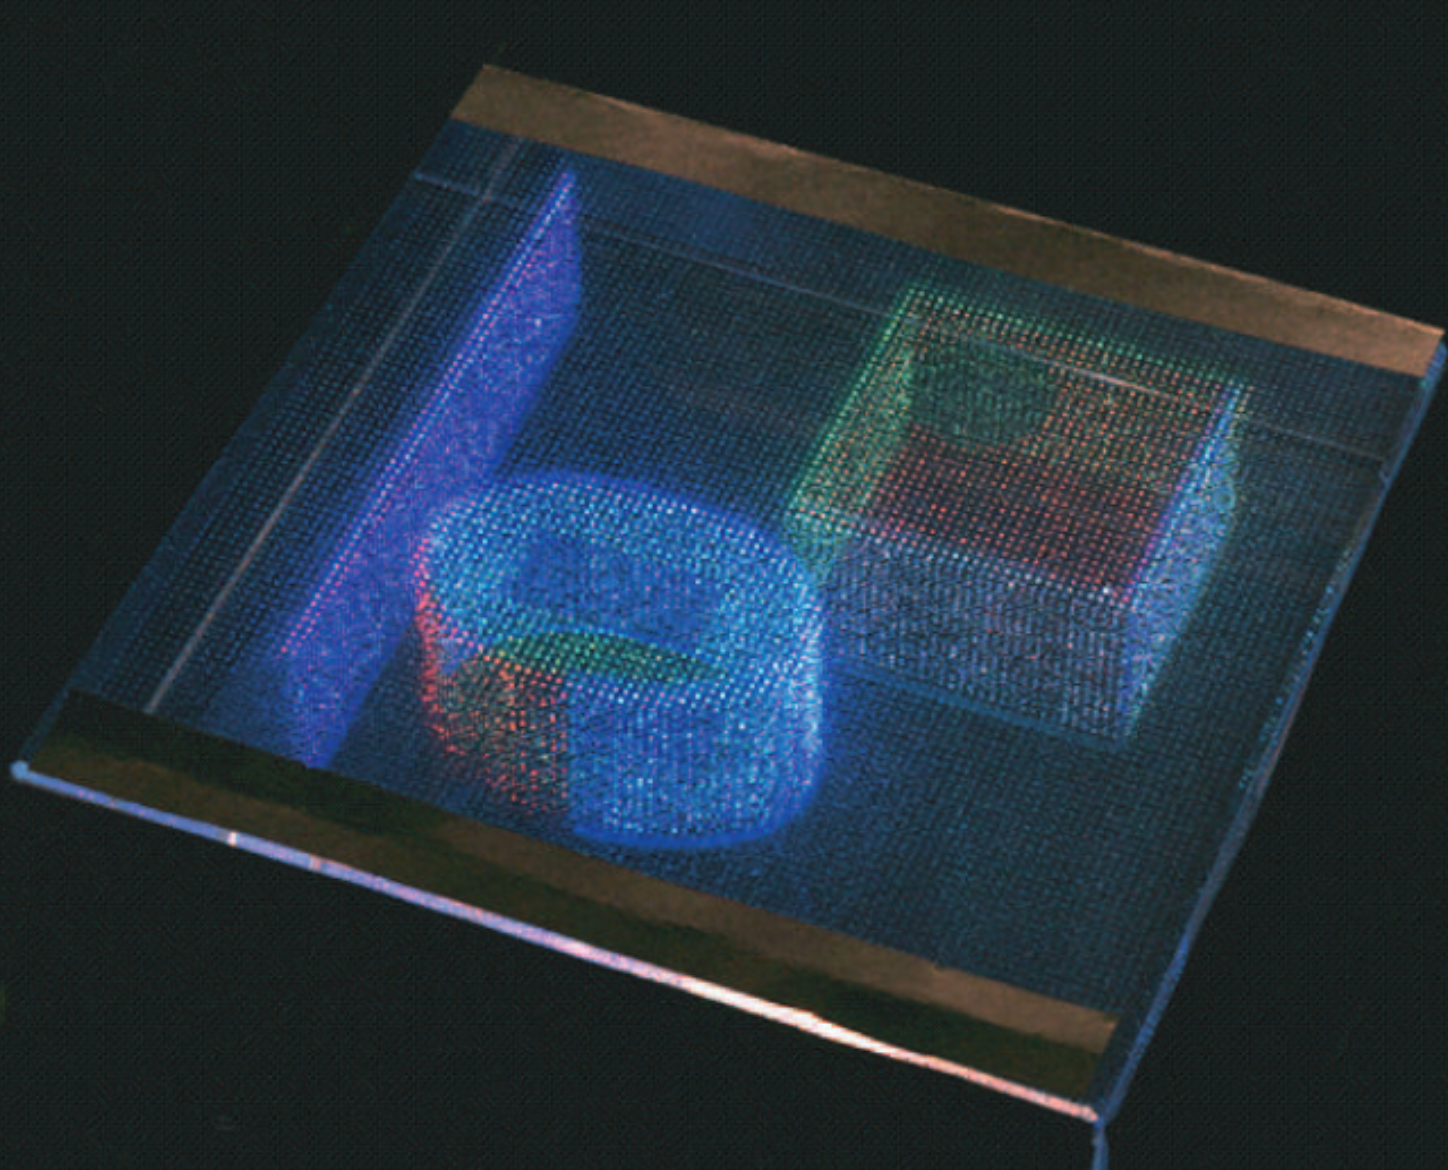
\includegraphics{./introduction/figures/passive optical scatterers.png}
	  }
	}
	\hfill
	\pictureBox[label={fig:acoustic}]{Bristol University's acoustic trapping volumetric display \cite{10.1063/1.5113467}}{
	\adjustbox{height=5.75cm, keepaspectratio}{
	  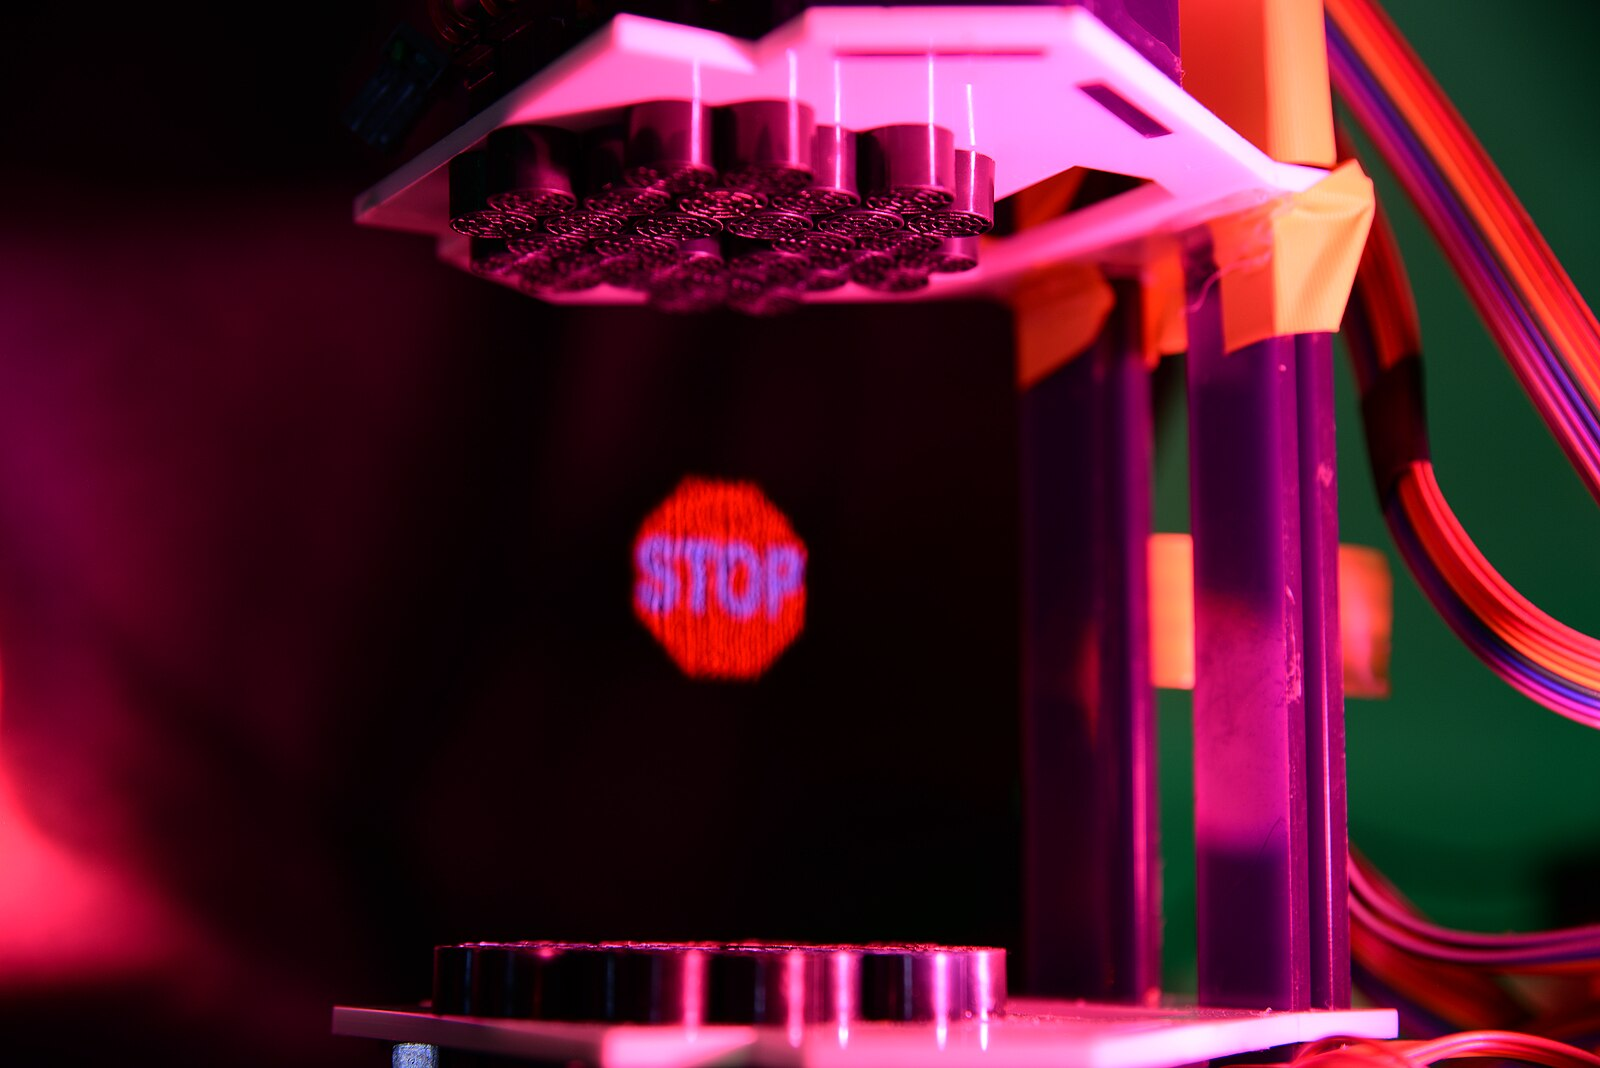
\includegraphics{./introduction/figures/acoustophoretic display.jpg}
	  }
	}
	\end{invisBox}
\subsection{Issues}

Volumetric displays often require custom/cutting-edge hardware (e.g. extremely high refresh rate projectors,  transparent micro LEDs, complex laser systems) which makes them expensive, difficult to manufacture and calibrate and not widely available. For example, the Voxon VX1, one of the few if only commercially available volumetric displays costs, \$11,700 USD \cite{noauthor_products_nodate} per unit. \\

Volumetric displays are also held back by their inherent high bandwidth requirements: To render objects in real-time at equivalent resolutions to current 2D displays while taking a raw voxel stream (as opposed to calculating voxels on hardware from primitive shapes) has an extremely high bandwidth requirement. If we want to render at \texttt{60fps} on a $4096 \times 2160 \times 1080$ voxel display with \texttt{24 bit} color, it would require a bandwidth of $1.37 \times 10^3$ bits per second/13.7 terabits per second which is orders of magnitude higher than what a normal display requires. To achieve that currently would require about 170 state-of-the-art Ultra High Bit Rate (UHBR) (80 gigabit) DisplayPort cables simultaneously. It was predicted in 2021 \cite{LAM2021050011} that due to these limitations and based on the historic trends of bandwidth in commercially available displays, volumetric displays will only become feasible in 2060 at the earliest. There are ways to reduce this bandwidth requirement through compression and other techniques \cite{4487481} but this still provides a major issue. \\

\subsection{Volumetric Screen Simulations}
Because of these issues, there has been some research into simulating volumetric displays. One commonly used method is the so-called fish tank virtual reality (FTVR) display \cite{10.1145/169059.169066} which has been commonly used to simulate volumetric displays, \cite{10.1145/3281505.3281540}, \cite{Zabarauskas2012}. A FTVR comprises a singular or set of 2D displays that are positioned in front of a user. The viewer's eyes are tracked in 3D space and the image on the displays is adjusted accordingly so that there appears to be a 3D image present in front of them. This is a relatively cheap and easy way to simulate a volumetric display, but it has some major drawbacks. The user is limited to a single focal depth and is limited to a single vergence (This can be fixed by wearing glasses to filter different images to each eye providing a stereo view \cite{5701756}). This system is also limited to just a single user at a time unless image filtering is used. 

Another approach that has been taken is to take advantage of virtual reality (VR) headsets. VR headsets are a relatively cheap and easy way to simulate a volumetric display. They are also able to provide a stereo view and can be used by multiple users at once \cite{10.1145/3290605.3300763}.
%%%%%%%%%%%%%%%%%%%%%%%%%%%%%%%%%%%%
\chapter{Contribution}


%%%%%%%%%%%%%%%%%%%%%%%%%%%%%%%%%%%%
\chapter{Experimental Results}


%%%%%%%%%%%%%%%%%%%%%%%%%%%%%%%%%%%%
\chapter{Conclusion}

%% bibliography
\printbibliography
\end{document}